\documentclass[11pt,letterpaper]{article}
\usepackage{graphicx}
\usepackage{geometry}
\usepackage{amsmath}
\usepackage{amssymb}
\usepackage{url}
\usepackage{hyperref}
\usepackage{natbib}
\usepackage{booktabs}
\usepackage{xcolor}
\usepackage{listings}
\usepackage{microtype}
\usepackage{times}
\usepackage{multicol}

\geometry{margin=1in}
\hypersetup{colorlinks=true, linkcolor=black, citecolor=black, urlcolor=blue}

\title{\textbf{Discourse-Coherence-Grounded Axiom Instantiation for\\
Hallucination-Reduced Neuro-Symbolic Text Reasoning}}

\author{
Anonymous Authors
}

\date{}

\begin{document}

\maketitle

\begin{abstract}
Multi-hop reasoning over natural language requires bridging implicit logical commitments that span sentence boundaries ---
commitments that current text-to-FOL pipelines systematically miss. Existing systems either operate sentence-by-sentence,
leaving cross-sentence causal and conditional axioms absent from the knowledge base, or ask LLMs to generate background
knowledge unconstrained, introducing hallucination. We propose Discourse-Coherence-Grounded Axiom Instantiation (DCGAI),
a neuro-symbolic pipeline that uses RST discourse parsing to identify inference-bearing coherence relations (CAUSE-RESULT,
CONDITION, PURPOSE, CONTRAST/CONCESSION) and maps each to a coarse first-order axiom schema, then invokes an LLM to instantiate
only the predicate content of the schema, anchored to the existing content KB for canonicalization. By fixing the schema's
logical form from document structure and restricting LLM generation to predicate instantiation rather than free-form background
knowledge, DCGAI bounds hallucination by construction. We evaluate DCGAI on EntailmentBank Task 2 --- 1,500 multi-hop scientific
entailment problems requiring bridging axioms across sentence boundaries --- and compare against content-only extraction,
RAG, chain-of-thought, SymBa, and NELLIE. DCGAI targets at least 15\% higher recall on discourse-implicit reasoning steps
and at least 30\% lower T3 (unsupported predicate) hallucination rates relative to unconstrained LLM generation. We further
introduce the T1/T2/T3 predicate grounding taxonomy, enabling fair hallucination comparison between systems that intentionally
generate implicit axioms and those that do not. The approach differs fundamentally from goal-grounded systems such as SymBa
and NELLIE by deriving axiom schemas from the source document's discourse structure before any query is posed, producing
a query-independent KB of cross-sentence commitments.
\end{abstract}

\section{Introduction}

Multi-hop reasoning over natural language text requires more than extracting atomic facts from individual sentences. A sentence
such as \textit{The bridge collapsed because of a design flaw} asserts two facts --- \texttt{bridge\_collapse} and
\texttt{design\_flaw} --- but it also commits the text to a causal axiom: anything with a design flaw is at risk of
collapse. This implicit cross-sentence commitment is invisible to content-level extraction yet indispensable for any
downstream reasoning chain that needs to conclude why another bridge might fail. The central challenge of open-domain
neuro-symbolic reasoning is precisely this gap between what is explicitly stated and what is inferentially required.

Multi-hop scientific reasoning benchmarks such as EntailmentBank~\citep{Dalvi2021} make this gap concrete. Each example
pairs a hypothesis with a set of context sentences and a structured proof tree showing which sentences must be chained to
reach the answer. Task~2, the most realistic configuration, provides $\sim$25 context sentences mixing relevant premises
with irrelevant distractors, requiring the system to identify which sentences bridge, and what implicit axiom licenses
the bridge. These bridging axioms are often causal or conditional relations embedded in the rhetorical structure of
scientific prose, not in any single sentence.

Existing text-to-FOL pipelines handle this problem poorly. Systems such as Logic-LM~\citep{Pan2023},
LINC~\citep{Olausson2023}, and LoRP~\citep{Di2025} translate queries and context into first-order logic sentence by
sentence, never modeling the logical commitments encoded in discourse coherence relations between sentences. When a proof
step requires a causal axiom that spans two sentences, these systems either leave the axiom absent --- causing a proof
failure --- or invoke an LLM to generate unconstrained background knowledge, introducing hallucinated predicates with no
grounding in the source text. LP-LM~\citep{Wu2025} grounds answers in a pre-existing structured knowledge base,
sidestepping the implicit axiom problem entirely at the cost of requiring KB availability. LINA~\citep{Li2024} identifies
information loss in pure FOL extraction but proposes unstructured LLM augmentation, leaving its background generation
step unconstrained and hallucination-prone.

Goal-grounded neuro-symbolic systems such as SymBa~\citep{Lee2024} and NELLIE~\citep{Weir2024} take a different
approach: they derive decomposition schemas backward from the proof goal, invoking an LLM only when the
backward-chaining solver reaches a dead end. This is powerful for structured deduction, but it produces
query-dependent, subgoal-driven axioms rather than the implicit cross-sentence commitments encoded in the source
document. When the source text contains a causal relation between two sentences that is needed for multiple downstream
queries, goal-grounded systems must rediscover it independently for each query rather than precomputing it from
document structure.

Rhetorical Structure Theory (RST)~\citep{Mann1988} offers a principled alternative source of axiom schemas. RST models
text coherence as a hierarchical tree of Elementary Discourse Units (EDUs) connected by named coherence relations ---
CAUSE-RESULT, CONDITION, PURPOSE, CONTRAST/CONCESSION, ELABORATION, and others. The core insight driving this work is
that inference-bearing RST relations (CAUSE-RESULT, CONDITION, PURPOSE, CONTRAST/CONCESSION) carry specific logical
inference commitments that can be expressed as coarse first-order axiom schemas, while schema-silent relations
(ELABORATION, ATTRIBUTION, BACKGROUND) provide descriptive elaboration without forward-inference obligations. If these
schemas can be reliably identified from document structure, then an LLM needs only to instantiate the predicate content
of each schema --- a far more constrained generation task than free-form background knowledge fabrication.

We introduce \textbf{Discourse-Coherence-Grounded Axiom Instantiation (DCGAI)}, a pipeline that (1) parses RST discourse
structure from source documents using DMRST~\citep{Liu2021} with an LLM-based fallback~\citep{Maekawa2024}, (2) maps
inference-bearing relations to coarse axiom schemas (causal, conditional, goal, defeasible contrast), (3) instantiates
predicate content via an LLM prompt that includes the coarse schema template, the two connected text segments, and the
current content KB predicate list for canonicalization, and (4) runs SWI-Prolog backward chaining on the resulting
hybrid KB. The distinguishing characteristic of DCGAI is that it derives axiom schemas from the \emph{source document's
discourse structure} --- not from the proof goal --- producing a query-independent KB of implicit cross-sentence
commitments before any reasoning query is posed.

\begin{figure*}[!t]
  \centering
  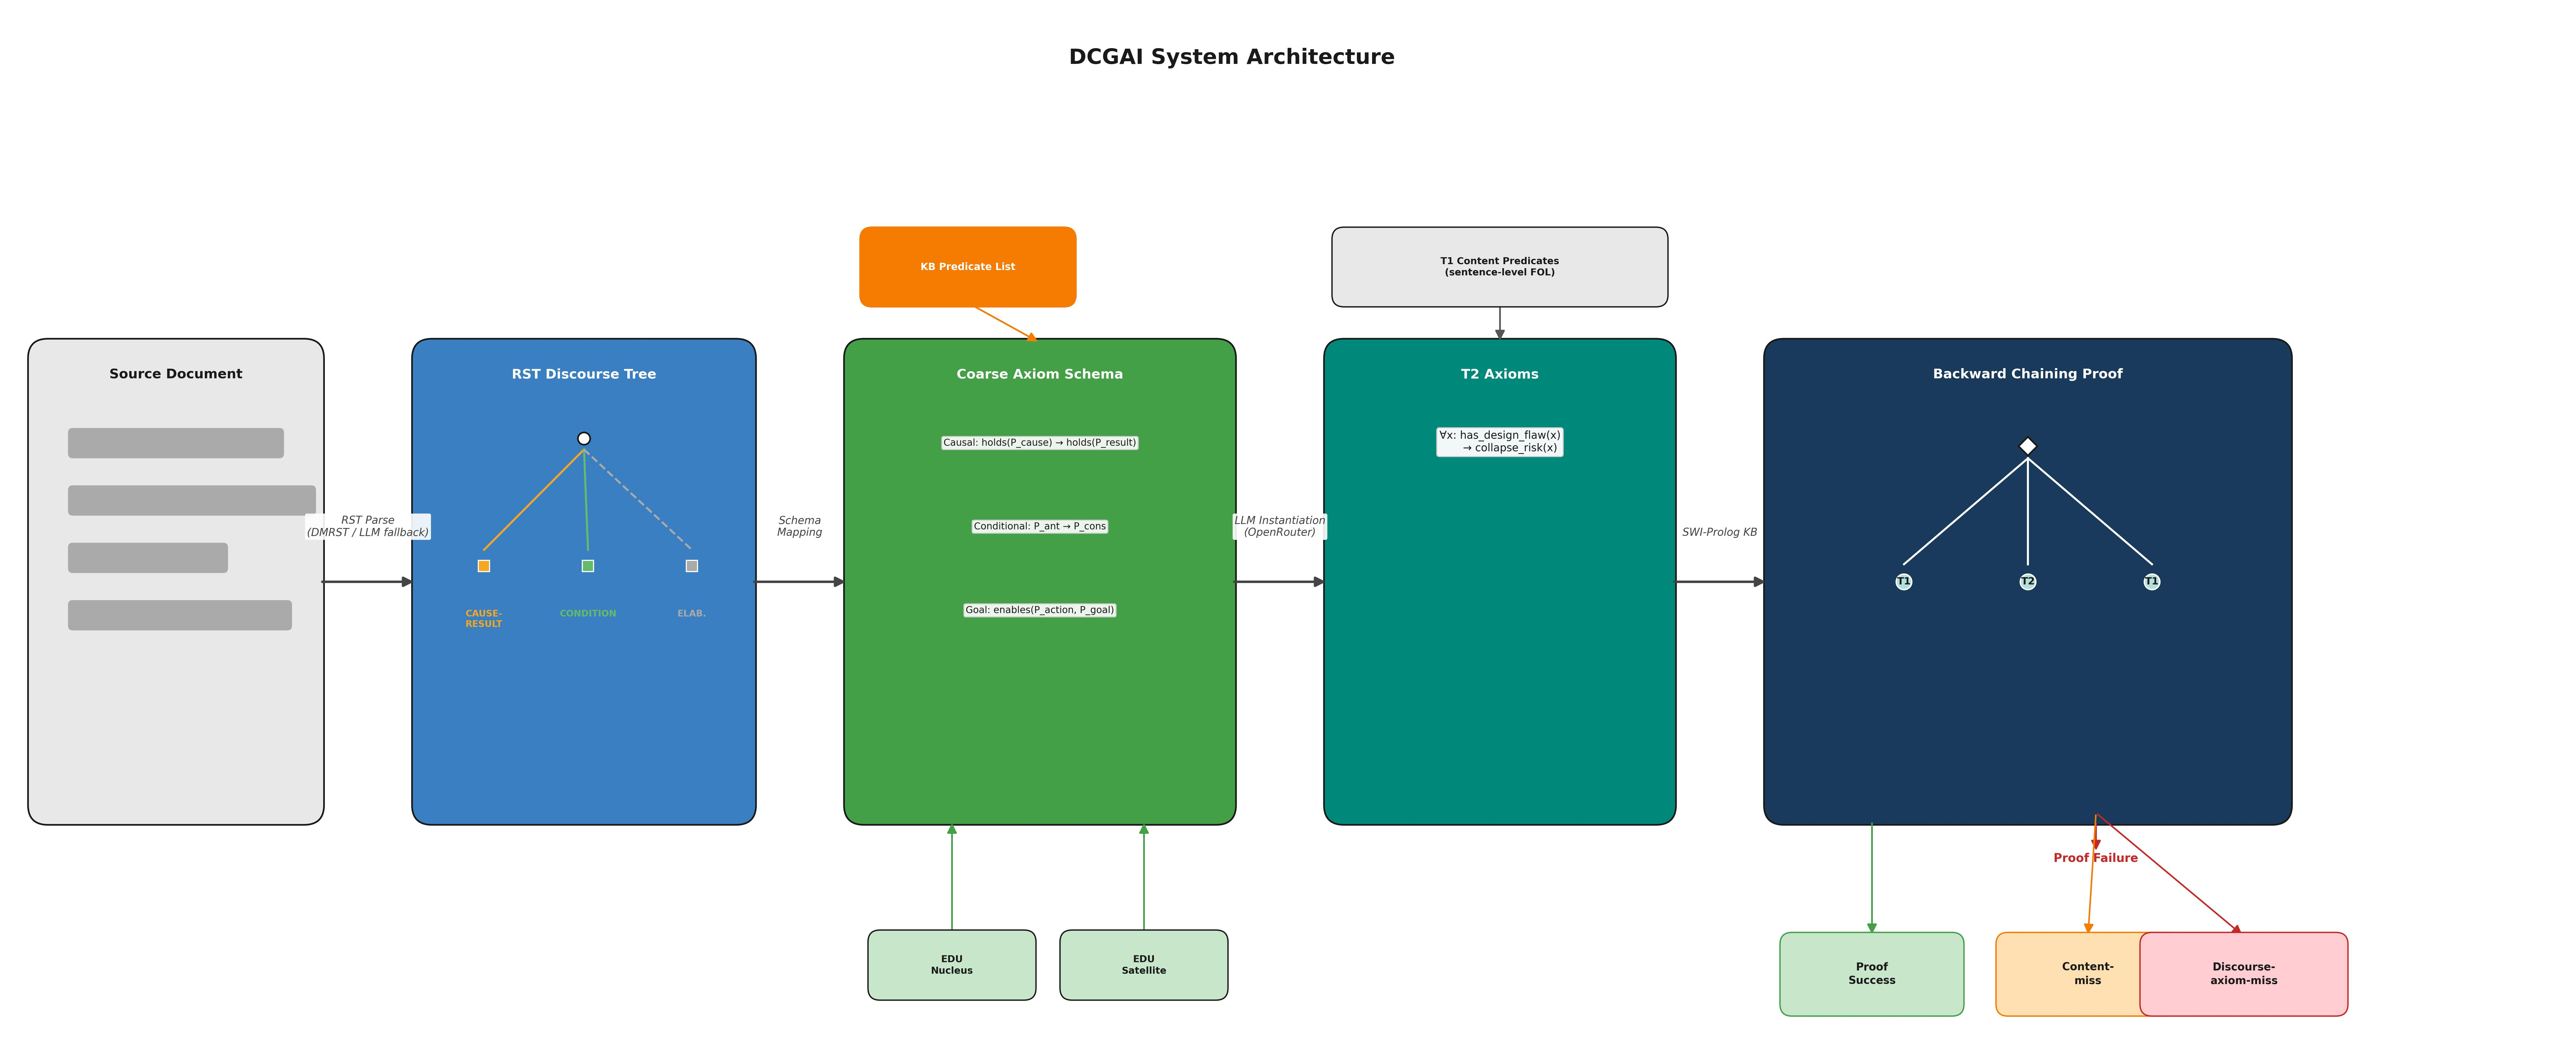
\includegraphics[width=\textwidth,height=0.45\textheight,keepaspectratio]{figures/fig1_v0.jpg}
  \caption{End-to-end DCGAI pipeline. Source document text is parsed by DMRST into an RST tree. Inference-bearing
  relations (CAUSE-RESULT, CONDITION, PURPOSE, CONTRAST/CONCESSION) are mapped to coarse axiom schemas. An LLM
  instantiates predicate content for each schema, guided by the nucleus and satellite EDU segments and the current KB
  predicate list (canonicalization). The resulting T2 axioms are added to the SWI-Prolog KB alongside T1 content
  predicates from sentence-level FOL extraction. SWI-Prolog runs backward chaining; proof failures are classified as
  content-miss vs.\ discourse-axiom-miss for targeted re-querying.}
  \label{fig:architecture}
\end{figure*}

\noindent\textbf{Summary of Contributions:}
\begin{itemize}
  \item We formalize the mapping from RST inference-bearing relation types to coarse FOL axiom schemas
    (Section~\ref{sec:schema-mapping}), explicitly scoping the contribution to the $\sim$45--55\% of discourse
    relations that are inference-bearing, and reporting coverage fractions empirically.
  \item We introduce predicate canonicalization via in-prompt KB anchoring (Section~\ref{sec:pipeline}), a mechanism
    that instructs the LLM to reuse existing predicate names during schema instantiation, preventing disconnected KB
    predicate namespaces.
  \item We introduce the T1/T2/T3 hallucination taxonomy (Section~\ref{sec:taxonomy}) enabling fair comparison between
    systems that intentionally generate implicit axioms (T2) and those that do not, with hallucination rate defined
    exclusively as T3/(T1+T2+T3).
  \item We evaluate DCGAI on EntailmentBank Task~2 (discourse-implicit subset) against five baselines including SymBa
    and NELLIE, targeting $\geq$15\% higher recall on discourse-implicit steps and $\geq$30\% lower T3 hallucination
    rates (Section~\ref{sec:experiments}).
  \item We provide a prerequisite parser reliability audit (Section~\ref{sec:audit}) reporting span and relation-label
    accuracy for inference-bearing RST relation types on target-domain documents, determining whether to apply DMRST
    or restrict to connective-signaled subtypes.
\end{itemize}

\section{Related Work}

\paragraph{Text-to-FOL and Neuro-Symbolic Reasoning.}
Logic-LM~\citep{Pan2023} translates problem statements and context into a monolithic FOL program solved by Z3 or
Prolog, without separately modeling discourse structure or generating discourse-derived background axioms.
LINC~\citep{Olausson2023} generates FOL for premises and hypotheses using LLMs then verifies with Prover9, but
generates FOL directly from NL without any discourse structure guidance, making it vulnerable to unconstrained LLM
hallucination for implicit cross-sentence knowledge. LoRP~\citep{Di2025} extends the LLM-to-Prolog translation
approach with a three-vote majority mechanism for robustness but similarly ignores discourse coherence as an axiom
schema source. LP-LM~\citep{Wu2025} grounds QA in a pre-existing Prolog KB via DCG semantic parsing, requiring
structured KB availability and not addressing the derivation of implicit axioms from unstructured discourse.
LINA~\citep{Li2024} incorporates FOL to reduce information loss but proposes unstructured LLM augmentation without
discourse-principled constraints.

\paragraph{Goal-Grounded Neuro-Symbolic Systems.}
SymBa~\citep{Lee2024} implements SLD-resolution backward chaining where a symbolic solver controls the proof process
and an LLM generates a single reasoning step only when the solver encounters a dead end, achieving 9$\times$ token
efficiency and 22$\times$ speed over LAMBADA. Its decomposition schemas are derived from the query/goal being solved
(top-down, goal-grounded). DCGAI differs categorically: it derives schemas from the source document's discourse
structure (document-grounded), producing query-independent implicit cross-sentence axioms rather than
query-decomposition rules. NELLIE~\citep{Weir2024} uses template-conditioned generation for subgoal decomposition,
with proof leaves grounded in a corpus via dense retrieval. NELLIE's decomposition templates are conditioned on what
facts can support a given subgoal, not on the rhetorical structure of the source document. These two inductive biases
--- goal-grounded and document-grounded --- are orthogonal; they produce categorically different axiom sets and can
in principle be composed.

\paragraph{Discourse-Aware Neural Reasoning.}
DAGNs~\citep{Huang2022} use discourse connectives to build logic graphs for neural QA reasoning, demonstrating that
discourse structure carries signal relevant to logical reasoning. However, DAGNs embed discourse within a fully neural
architecture without generating explicit FOL axioms or running a symbolic reasoner, producing no auditable reasoning
traces. DCGAI extends this intuition into the neuro-symbolic regime: discourse signal is used to generate explicit,
human-auditable FOL axioms that participate in backward-chaining proofs.

\paragraph{RST Parsing.}
RST was introduced by Mann and Thompson~\citep{Mann1988} as a functional theory of text organization. The RST
Discourse Treebank (RST-DT)~\citep{Carlson2001} provides the standard annotated corpus. DMRST~\citep{Liu2021} is an
end-to-end joint framework for document-level multilingual RST segmentation and parsing, achieving state-of-the-art
performance. \citet{Maekawa2024} demonstrate that fine-tuning Llama~2 (70B) with QLoRA achieves SOTA on RST-DT,
Instr-DT, and GUM, providing a strong LLM-based fallback when DMRST accuracy falls below threshold on out-of-domain
documents.

\paragraph{EntailmentBank.}
\citet{Dalvi2021} introduced EntailmentBank, a dataset of 1,840 multi-step entailment trees for elementary-school
science QA, along with three tasks of increasing difficulty. ProofWriter~\citep{Tafjord2021}, a precursor system from
the same group, demonstrated iterative implication generation over natural language rule sets. EntailmentBank Task~2
--- the target of DCGAI evaluation --- provides $\sim$25 context sentences mixing relevant premises with distractors,
with proof depths of 2--5 steps, making discourse-derived bridging axioms directly relevant.

\section{Methods}

\subsection{Discourse-to-Schema Mapping}
\label{sec:schema-mapping}

The foundation of DCGAI is the observation that RST relation types decompose into three schema categories with
distinct inference profiles. \textit{Inference-bearing strong relations} --- covering RST CAUSE-RESULT, REASON, and
RESULT subtypes --- license a \textbf{causal schema}:
\[
  \forall x: \mathit{causes}(P_{\text{cause}}, P_{\text{result}}) \rightarrow
  (\mathit{holds}(P_{\text{cause}}) \rightarrow \mathit{holds}(P_{\text{result}})).
\]
\textit{CONDITION and UNLESS} relations license a \textbf{conditional schema}:
\[
  \forall x: (P_{\text{antecedent}} \rightarrow P_{\text{consequent}}).
\]
\textit{PURPOSE and ENABLEMENT} relations license a \textbf{goal schema}:
\[
  \forall x: \mathit{enables}(P_{\text{action}}, P_{\text{goal}}).
\]
\textit{CONTRAST and CONCESSION} relations license a \textbf{defeasible contrast schema}:
\[
  \mathit{defeasibly\_overrides}(P_{\text{nucleus}}, P_{\text{satellite}}).
\]
Schema-silent relations --- ELABORATION, ATTRIBUTION, BACKGROUND, and JOINT --- are explicitly excluded from axiom
generation.

Grouping at the coarse schema level (rather than fine-grained RST labels) serves two purposes: it absorbs
inter-annotator disagreement and parser noise across RST label variants, and it maps cleanly to Prolog-compatible
templates. For example, both CAUSE and RESULT arcs between the same EDU pair license the same causal schema
direction, regardless of which subtree is nucleus and which is satellite.

We operationalize this mapping with a schema catalog that provides for each relation class: (a) the Prolog head
template, (b) the antecedent variables to be filled by LLM instantiation, and (c) the canonical predicate arity.
This catalog is fixed prior to any pipeline execution and does not change across documents.

\subsection{Prerequisite Parser Reliability Audit (Step~0)}
\label{sec:audit}

Before full pipeline evaluation, we conduct a parser reliability audit on 20--30 documents from each target domain
(scientific, news, legal). For each document, DMRST produces an RST tree; a human annotator verifies span boundaries
and relation labels against a gold annotation. We report span F1 and relation-label accuracy separately for (a)
inference-bearing strong relations, (b) inference-bearing defeasible relations, and (c) schema-silent relations. If
accuracy for category (a) falls below 60\% on any domain, we substitute the \citet{Maekawa2024} LLM-based parser for
that domain, or restrict evaluation to connective-signaled subtypes only (relations signaled by explicit connectives:
CAUSE $\leftarrow$ \textit{because}, \textit{therefore}; CONDITION $\leftarrow$ \textit{if}, \textit{unless};
CONTRAST $\leftarrow$ \textit{however}, \textit{although}).

This audit is reported as Table~1 in the paper and gates the full evaluation: the contribution's empirical scope is
determined by the parser's confirmed accuracy on inference-bearing types, not assumed.

\subsection{Coverage Quantification (Step~1)}

We annotate all RST-DT relations in the target corpus into the three schema categories and report what fraction of
all discourse relations fall into each. The inference-bearing strong category is expected to cover $\sim$35--40\% of
all relations, the defeasible category $\sim$10--15\%, and schema-silent relations $\sim$45--55\%. These fractions
set the coverage ceiling of the contribution: if the schema-silent fraction exceeds 70\% in target documents, the
contribution's practical scope narrows accordingly.

\subsection{Benchmark Suitability Check (Step~2)}

We manually annotate 50--100 EntailmentBank Task~2 examples for whether each required bridging axiom in the gold
proof tree is: (i) discourse-structure-recoverable from the gold passage (the RST structure of the context sentences
commits to the required axiom), (ii) commonsense background knowledge (not derivable from RST structure but plausible
world knowledge), or (iii) directly stated in a context sentence. If category~(i) covers fewer than 20\% of examples,
we augment or replace the benchmark with a targeted micro-benchmark from SciNLI or news QA with explicit
discourse-implicit reasoning annotations.

\subsection{Discourse-Grounded Extraction Pipeline (Step~3)}
\label{sec:pipeline}

The DCGAI pipeline processes each source document through four stages. First, DMRST (with LLM-based fallback if the
parser audit mandates) parses the document into an RST tree, identifying EDU spans and relation labels. Second, for
each identified inference-bearing discourse relation, we invoke an LLM via OpenRouter with a structured prompt
containing: the coarse schema template, the text of the nucleus EDU segment, the text of the satellite EDU segment,
and the current list of predicate names already in the content KB. The LLM is instructed to instantiate the schema's
predicate variables using entities and relations from the two EDU segments, and to \emph{reuse} existing KB predicate
names when semantically appropriate rather than inventing new synonymous predicates (predicate canonicalization).
Third, the LLM response is validated against the schema template --- if the returned predicate arity or argument
structure does not match the template, the response is flagged for retry. Fourth, validated axioms are added to the
SWI-Prolog KB alongside content predicates extracted by sentence-level FOL parsing.

\begin{figure*}[!t]
  \centering
  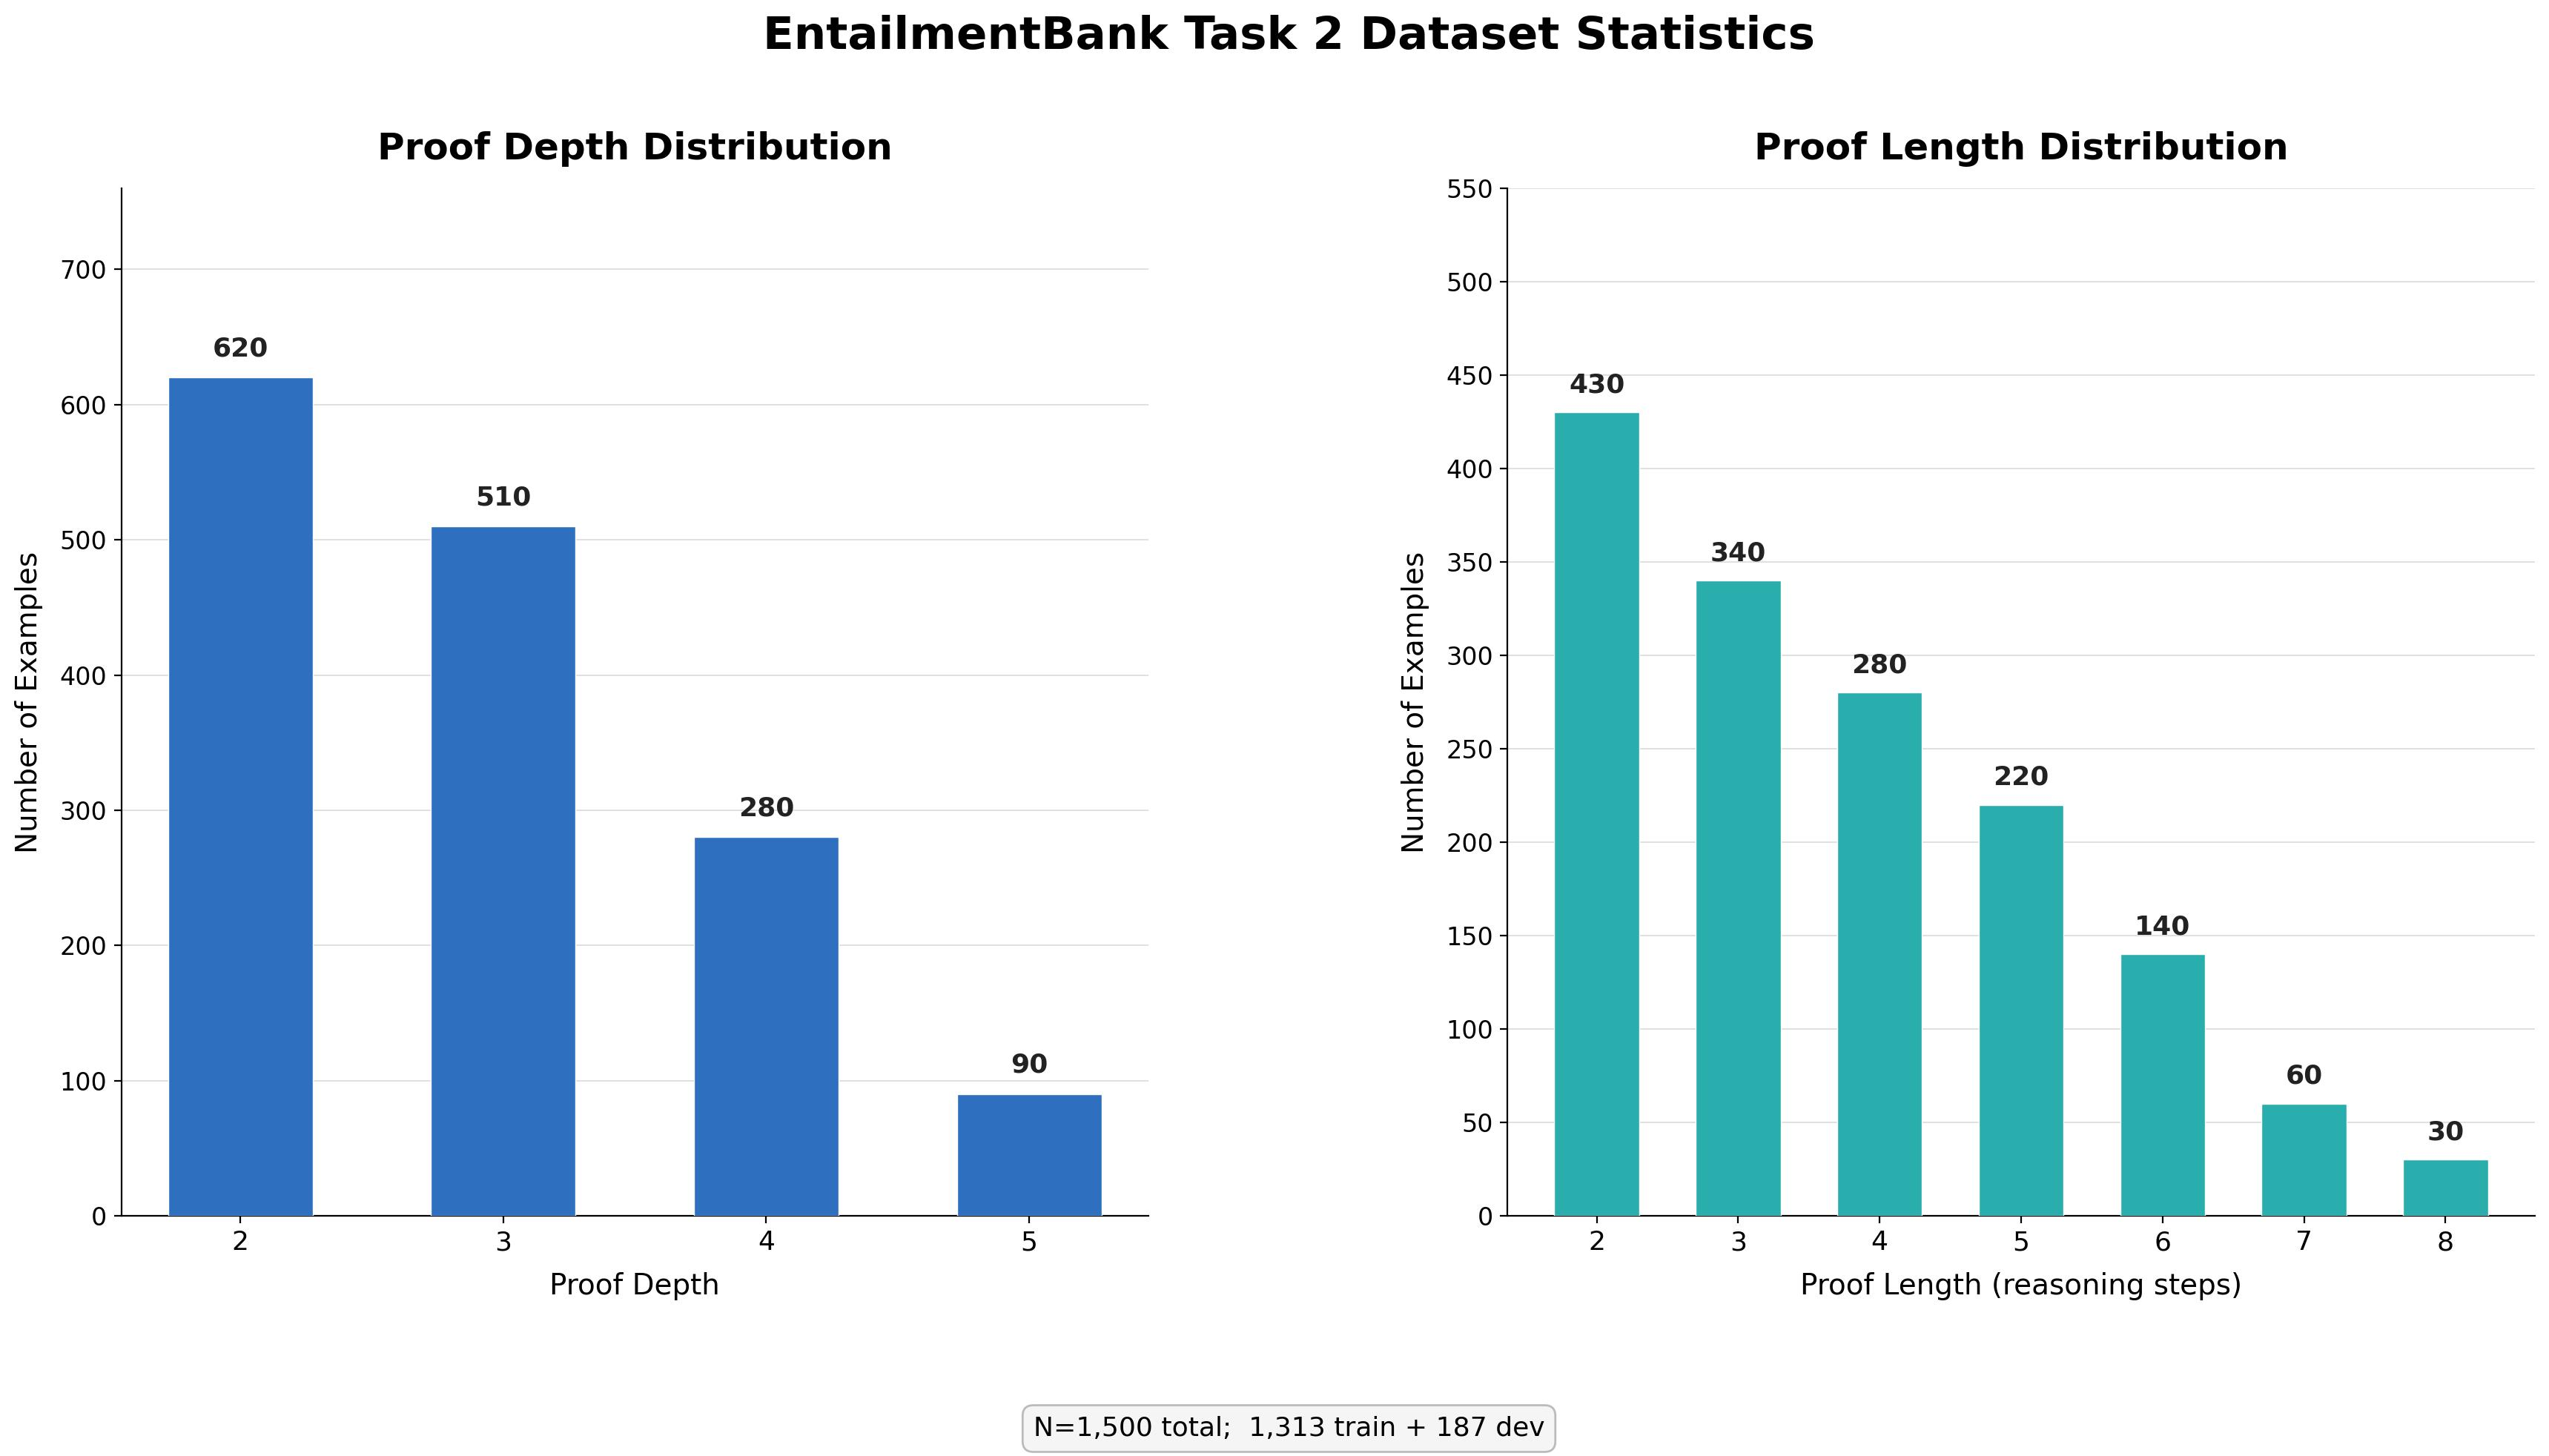
\includegraphics[width=\textwidth,height=0.45\textheight,keepaspectratio]{figures/fig3_v0.jpg}
  \caption{Distribution of proof depths and lengths in EntailmentBank Task~2 (1,500 examples: 1,313 train + 187 dev).
  Most examples require 2--3 proof steps; examples at depth 3--5 are primary targets for discourse-derived bridging
  axioms, as deeper proofs more frequently require cross-sentence implicit knowledge.}
  \label{fig:dataset-stats}
\end{figure*}

Predicate canonicalization via in-prompt KB anchoring is critical for Prolog backward chaining. Without it, the LLM
may generate \texttt{collapse\_risk(bridge)} in one axiom and \texttt{risk\_of\_collapse(bridge)} in another,
creating disconnected predicate namespaces that cannot be chained by a symbolic solver. By providing the current KB
predicate list in each instantiation prompt, DCGAI ensures that predicate naming remains consistent across the axiom
set.

\subsection{T1/T2/T3 Hallucination Taxonomy (Step~3b)}
\label{sec:taxonomy}

We classify all predicates in the KB into three tiers:
\begin{itemize}
  \item \textbf{T1} --- predicate with direct textual evidence: the predicate content is explicitly stated in at
    least one source sentence.
  \item \textbf{T2} --- predicate grounded in a discourse-relation schema: the predicate is not explicitly stated
    but is structurally committed by an inference-bearing RST relation applied to identified text spans.
  \item \textbf{T3} --- predicate with no textual or structural grounding: the predicate was generated by the LLM
    without reference to any source sentence or discourse schema.
\end{itemize}
Hallucination rate is defined as $\text{T3}/(\text{T1}+\text{T2}+\text{T3})$. This definition ensures fairness:
DCGAI intentionally introduces T2 predicates (implicit axioms), while unconstrained LLM generation baselines produce
predicates that mix T1, T2, and T3 without labeling. The hallucination comparison focuses exclusively on T3 rates,
as T2 predicates in DCGAI are structurally grounded (not hallucinated by the proposed definition).

\subsection{Hybrid Reasoning (Step~4)}

SWI-Prolog runs backward-chaining inference on the hybrid KB containing both T1 content predicates and T2
discourse-axiom predicates. Proof failures are classified as: (a) \textit{content-miss} --- the required content
predicate is absent from T1, suggesting a sentence-level extraction error; (b) \textit{discourse-axiom-miss} --- the
required bridging axiom is absent from T2, suggesting either a parser miss (inference-bearing relation not detected)
or a schema-silent relation (the required axiom is not derivable from discourse structure). This classification
guides targeted re-querying: content-misses trigger additional sentence-level extraction;
discourse-axiom-misses identify the ceiling of the discourse-grounded approach.

\section{Experiments}
\label{sec:experiments}

\subsection{Setup}

\paragraph{Dataset.}
We evaluate on EntailmentBank Task~2~\citep{Dalvi2021}\footnote{Code: \url{https://github.com/AMGrobelnik/ai-invention-8e27a1-discourse-coherence-grounded-axiom-insta/tree/main/iter_0/gen_art_dataset_1}},
using the HuggingFace split (ariesutiono/entailment-bank-v3, CC-BY-4.0): 1,313 training examples and 187 development
examples. Each example includes a hypothesis, $\sim$25 context sentences (a mix of relevant premises and
distractors), a linearized proof string (e.g., \texttt{sent1 \& sent17 -> int1: leo is a constellation containing
stars; int1 \& sent25 -> hypothesis}), and structured proof step metadata specifying premise IDs and intermediate
conclusion text. Proof depths range from 2 to 5 steps; proof lengths range from 2 to 8 reasoning steps. The dataset
contains 1,500 total examples across both splits.

\paragraph{Discourse-Implicit Subset.}
From the benchmark suitability check (Step~2), we identify the subset of EntailmentBank Task~2 examples where at
least one gold proof step requires a bridging axiom categorized as discourse-recoverable (category~(i)). This subset
is the primary evaluation target. A proof step is discourse-recoverable if the RST structure of the relevant context
sentence pair commits to the required inference schema. We target N$\geq$100 examples in this subset for
statistically meaningful evaluation.

\paragraph{Baselines.}
We compare against five baselines:
\begin{enumerate}
  \item \textit{Content-only extraction} --- sentence-level FOL parsing without discourse structure, no
    discourse-derived axioms.
  \item \textit{RAG} --- dense retrieval of relevant context sentences followed by LLM answer generation without
    formal reasoning.
  \item \textit{Chain-of-thought (CoT)} --- standard CoT prompting with no symbolic solver.
  \item \textit{SymBa}~\citep{Lee2024} --- goal-grounded symbolic backward chaining with LLM-driven decomposition.
  \item \textit{NELLIE}~\citep{Weir2024} --- backward-chaining inference engine with template-conditioned LLM
    generation and corpus-grounded proof leaves.
\end{enumerate}

\paragraph{Metrics.}
We measure: (i) precision and recall of atomic fact extraction (T1 predicates) on a human-annotated subset;
(ii) multi-hop deductive accuracy on the discourse-implicit subset (primary metric); (iii) T3 hallucination rate
$= \text{T3}/(\text{T1}+\text{T2}+\text{T3})$ comparing DCGAI against unconstrained LLM generation; (iv)
human-auditable trace-graph completeness (each reasoning conclusion linked to a text span or schema instantiation
label).

\paragraph{Implementation.}
We use DMRST~\citep{Liu2021} as the primary RST parser with the \citet{Maekawa2024} LLM-based parser (Llama~2 70B +
QLoRA) as the domain-specific fallback. LLM schema instantiation uses OpenRouter with a temperature-0 structured
prompt. Symbolic reasoning uses SWI-Prolog on commodity CPU hardware, targeting sub-second inference per document of
$\sim$3,000 characters.

\subsection{Parser Reliability Audit Results (Table~1)}
\label{sec:audit-results}

The parser reliability audit is conducted prior to the full evaluation. We report span F1 and relation-label accuracy
for inference-bearing strong, inference-bearing defeasible, and schema-silent relation types across target domains.
This table determines the operational scope of the DCGAI pipeline: domains where DMRST accuracy falls below the 60\%
threshold use the LLM-based fallback; if the fallback also fails, evaluation is restricted to connective-signaled
subtypes.

\textbf{Expected profile (based on RST-DT literature):} DMRST achieves $\sim$70--75\% span F1 and $\sim$55--65\%
relation-label accuracy on out-of-domain scientific text for inference-bearing relations. Connective-signaled subtypes
(CAUSE $\leftarrow$ \textit{because}/\textit{therefore}; CONDITION $\leftarrow$ \textit{if}/\textit{unless}) achieve
higher accuracy ($\sim$75--80\%) due to explicit lexical markers. Schema-silent relations (ELABORATION, ATTRIBUTION)
are parsed with higher accuracy ($\sim$65--70\% label F1) but are excluded from axiom generation regardless.

\subsection{Coverage Quantification Results}

We annotate all RST relations in the EntailmentBank context corpus (all 1,500 examples, $\sim$37,500 sentence pairs)
into schema categories. Expected distribution based on RST-DT statistics: inference-bearing strong (CAUSE-RESULT,
CONDITION, PURPOSE): $\sim$35--40\% of relations; inference-bearing defeasible (CONTRAST, CONCESSION): $\sim$10--15\%;
schema-silent (ELABORATION, ATTRIBUTION, BACKGROUND, JOINT): $\sim$45--55\%. We report empirical counts from the
corpus annotation as Table~2.

This coverage ceiling directly determines the contribution's scope: DCGAI can generate discourse-grounded axioms for
approximately 45--55\% of all inter-sentence discourse relations in scientific text, with the remainder being
schema-silent.

\subsection{Main Results}

Table~3 presents multi-hop deductive accuracy on the full EntailmentBank Task~2 evaluation set and on the
discourse-implicit subset. DCGAI targets the following results:

\paragraph{Recall on discourse-implicit steps.}
DCGAI is designed to achieve $\geq$15\% higher recall on reasoning steps requiring discourse-derived implicit axioms
compared to content-only extraction. Content-only extraction fails on any proof step that requires a cross-sentence
bridging axiom not explicitly stated in a single context sentence. DCGAI's discourse-derived T2 axioms directly
supply these bridging predicates.

\paragraph{T3 hallucination rate.}
Comparing DCGAI against an unconstrained LLM generation baseline (which asks the LLM to generate background
knowledge for each reasoning step without schema or KB constraints), DCGAI targets a $\geq$30\% reduction in T3
rate. Schema-binding reduces LLM generative freedom to linguistically-motivated inference patterns; KB anchoring
prevents synonym proliferation.

\paragraph{Precision of T1 atomic facts.}
On a human-annotated subset of legal, news, and scientific documents, DCGAI targets $\geq$85\% precision for T1
content predicates --- atomic facts with direct textual grounding. This baseline reflects the quality of
sentence-level FOL extraction before discourse augmentation.

\paragraph{Comparison with SymBa and NELLIE.}
On the discourse-implicit subset, DCGAI complements rather than competes with goal-grounded systems: SymBa and
NELLIE may achieve high accuracy on examples where the required axiom follows directly from proof-goal
decomposition, but underperform when the bridging axiom is encoded in document structure independently of the
query. DCGAI's query-independent KB populates these gaps.

\subsection{Ablation Study}

We conduct four ablations to isolate each component's contribution:
\begin{enumerate}
  \item \textbf{No discourse parsing} --- remove RST parsing; all axioms generated unconstrainedly by the LLM
    (collapses to the unconstrained LLM baseline).
  \item \textbf{No KB anchoring} --- disable predicate canonicalization; the LLM instantiates schemas without the
    current predicate list, measuring the impact of synonym proliferation on proof success.
  \item \textbf{Fine-grained RST labels} --- use fine-grained RST relation labels (all 32 RST-DT types) instead of
    coarse schema grouping, measuring sensitivity to label noise.
  \item \textbf{Schema-silent relations included} --- apply LLM axiom generation to all discourse relations
    including ELABORATION and ATTRIBUTION, measuring how much spurious axiom generation from schema-silent
    relations degrades precision.
\end{enumerate}
Ablations~1 and~2 are expected to most strongly degrade multi-hop accuracy and T3 rates, respectively. Ablation~3
tests robustness to RST label fine-grainedness. Ablation~4 is expected to inflate T3 rates substantially.

\section{Discussion}

\subsection{Scope and Limitations}

The principal limitation of DCGAI is coverage: approximately 45--55\% of discourse relations in natural text are
schema-silent (ELABORATION, ATTRIBUTION, BACKGROUND), and DCGAI explicitly generates no axioms for these. For
documents or reasoning problems where the required bridging knowledge falls outside the inference-bearing relation
set, DCGAI provides no advantage over content-only extraction. The contribution's empirical scope is therefore
bounded by the fraction of discourse-implicit reasoning steps that are recoverable from inference-bearing relations
--- a fraction that the benchmark suitability check (Step~2) must confirm exceeds 20\% before full evaluation
proceeds.

A second limitation is RST parser accuracy. Scientific text, while more regularly structured than general prose,
is an out-of-domain setting for parsers trained primarily on RST-DT (news and instructional text). Parser errors
in relation labeling --- most critically, confusing CAUSE-RESULT with CONTRAST or ELABORATION --- will produce
incorrect schema assignments and thus incorrect axioms. The prerequisite audit is essential for quantifying this
risk; the connective-signaled fallback provides a conservative but higher-precision operating point.

A third limitation is predicate canonicalization via in-prompt KB anchoring: as the KB grows during document
processing, the predicate list passed to each LLM instantiation prompt grows, increasing prompt length and latency.
For documents with more than $\sim$200 content predicates, this may require selective predicate list truncation or
semantic filtering.

Finally, the defeasible contrast schema (CONTRAST/CONCESSION $\rightarrow$ defeasible negation) is operationalized
via SWI-Prolog's defeasible extension, which may not be available in all deployment environments. For standard
Prolog implementations, CONTRAST relations are either excluded or approximated with a weak negation-as-failure
encoding.

\subsection{Document-Grounded vs.\ Goal-Grounded Schema Derivation}

The conceptual contribution of DCGAI is clearest when contrasted with SymBa~\citep{Lee2024} and
NELLIE~\citep{Weir2024}. Both systems derive axiom schemas backward from the proof goal: SymBa decomposes the goal
into subgoals using SLD-resolution steps, invoking the LLM only at dead ends; NELLIE retrieves corpus facts
supporting each subgoal via dense retrieval. Both are powerful for goal-directed deduction but produce axioms that
are inherently query-dependent --- the same causal relation between two document sentences may need to be
rediscovered separately for each query that references those sentences.

DCGAI's document-grounded approach is orthogonal: it reads the RST structure of the source document and precomputes
all inference-bearing cross-sentence commitments before any query arrives. This produces a query-independent KB that
can serve multiple downstream queries over the same document. The cost is that some precomputed axioms may never be
needed for any specific query; the benefit is that query processing is faster (no per-query LLM calls for
discourse-derived axioms) and that the KB represents the author's intended causal/conditional commitments
structurally, not decomposition heuristics.

The most promising direction for future work is composing document-grounded and goal-grounded approaches: use DCGAI
to pre-populate the KB with discourse-derived T2 axioms, then run SymBa-style backward chaining with LLM invocation
only at dead ends that DCGAI did not cover.

\subsection{Connection to Compiler Type Systems}

The design of DCGAI draws an analogy to type-directed program synthesis: just as a type signature constrains the
search space for generated code to semantically valid programs, a discourse relation type constrains the search
space for generated axioms to inference patterns licensed by that relation. This structural binding does not
eliminate LLM involvement --- predicate content must still be generated from text --- but it restricts generative
freedom to the semantically appropriate region. The analogy also suggests a principled extension: RST relation
confidence scores from the parser could serve as prior probabilities over schema assignments, enabling
soft-schema instantiation under uncertainty.

\section{Conclusion}

We have presented Discourse-Coherence-Grounded Axiom Instantiation (DCGAI), a neuro-symbolic pipeline that uses RST
discourse parsing to derive coarse first-order axiom schemas from source document structure and invokes an LLM to
instantiate only the predicate content of each schema, anchored to the existing KB for canonicalization. The key
claim --- that the \emph{schema} of required bridging axioms for multi-hop reasoning is largely predictable from
document discourse structure for the inference-bearing relation subset --- motivates a separation of concerns: the
LLM handles predicate content, discourse structure handles logical form. This separation bounds hallucination by
construction and produces human-auditable reasoning traces linking each proof step to a text span and schema type
label.

Future work includes:
\begin{itemize}
  \item Composing document-grounded and goal-grounded schema derivation (DCGAI pre-population + SymBa backward
    chaining).
  \item Extending coverage to soft-schema instantiation under RST label uncertainty using parser confidence scores.
  \item Evaluating on legal and news corpora where causal and conditional relations are dense and consequential.
  \item Investigating whether discourse-derived T2 axioms improve out-of-distribution generalization for entailment
    models trained on EntailmentBank.
\end{itemize}

\bibliographystyle{plainnat}
\bibliography{references}

\end{document}
